\documentclass[11pt,a4paper]{article}
%\usepackage{mathtools,comicsans}
%\usepackage{babel}
\usepackage[utf8]{inputenc}
\usepackage[left=2.5cm,right=2cm, bottom=2cm]{geometry}
\usepackage{amsmath}
\usepackage{amsfonts}
\usepackage{amssymb}
\usepackage{amsfonts}
\usepackage{amsmath}
\usepackage{graphicx}
\usepackage{import}
%\usepackage{subfig}
\usepackage{subcaption}
\usepackage{multirow}
\usepackage{color}
\usepackage{abstract}
\usepackage{braket}
\usepackage{float}
\usepackage[toc,page]{appendix}
%\usepackage{url}
\usepackage{hyperref}

\usepackage{tabularx}
%\usepackage{subfigure}
\usepackage{listings}
\DeclareUnicodeCharacter{2212}{-}
\graphicspath{ {./res/} } % Sets path to folder with images/figures

\setlength {\marginparwidth }{2cm}
\usepackage{todonotes}

\usepackage{biblatex}
\addbibresource{bibliography.bib}


%\renewcaptionname\figureautorefname{Fig.}
\renewcommand{\figureautorefname}{Fig.}
\renewcommand{\figurename}{Fig.}

\newcommand{\overbar}[1]{\mkern 1.5mu\overline{\mkern-1.5mu#1\mkern-1.5mu}\mkern 1.5mu}

%% Algorithm
\usepackage{listings}
\lstset{language=C++}
\lstset{
        mathescape=true,
        morekeywords={if,then,else,return}
        }
\lstset{ 
    captionpos=t,
    tabsize=2
}
\lstset{basicstyle=\ttfamily\footnotesize,breaklines=true}
\renewcommand{\lstlistingname}{Algorithm}% Listing -> Algorithm
\renewcommand{\lstlistlistingname}{List of \lstlistingname s}% List of Listings -> List of Algorithms

\lstset{
    frame=tb, % draw a frame at the top and bottom of the code block
    tabsize=4, % tab space width
    showstringspaces=false, % don't mark spaces in strings
    numbers=left, % display line numbers on the left
    commentstyle=\color{green}, % comment color
    keywordstyle=\color{blue}, % keyword color
    stringstyle=\color{red} % string color
    basicstyle=\footnotesize\ttfamily
}

\author{Hiti Mario, 01327428}
\date{\today}
\title{Computational Science on Many-Core Architectures - Ex9}


% double underline
\def\doubleunderline#1{\underline{\underline{#1}}}

\begin{document}
%%%%%%%%% TITLE PAGE %%%%%%%%%
\maketitle

\newpage
\tableofcontents
%\listoftodos

\thispagestyle{empty}
\newpage
\setcounter{page}{1}


%%%%%%%%% Begin Document %%%%%%%%%
% \include{1-Introduction}
%\include{2-conjugate-gradients}
\section{Is this the real life?}



\begin{figure}[H]
	\centering
	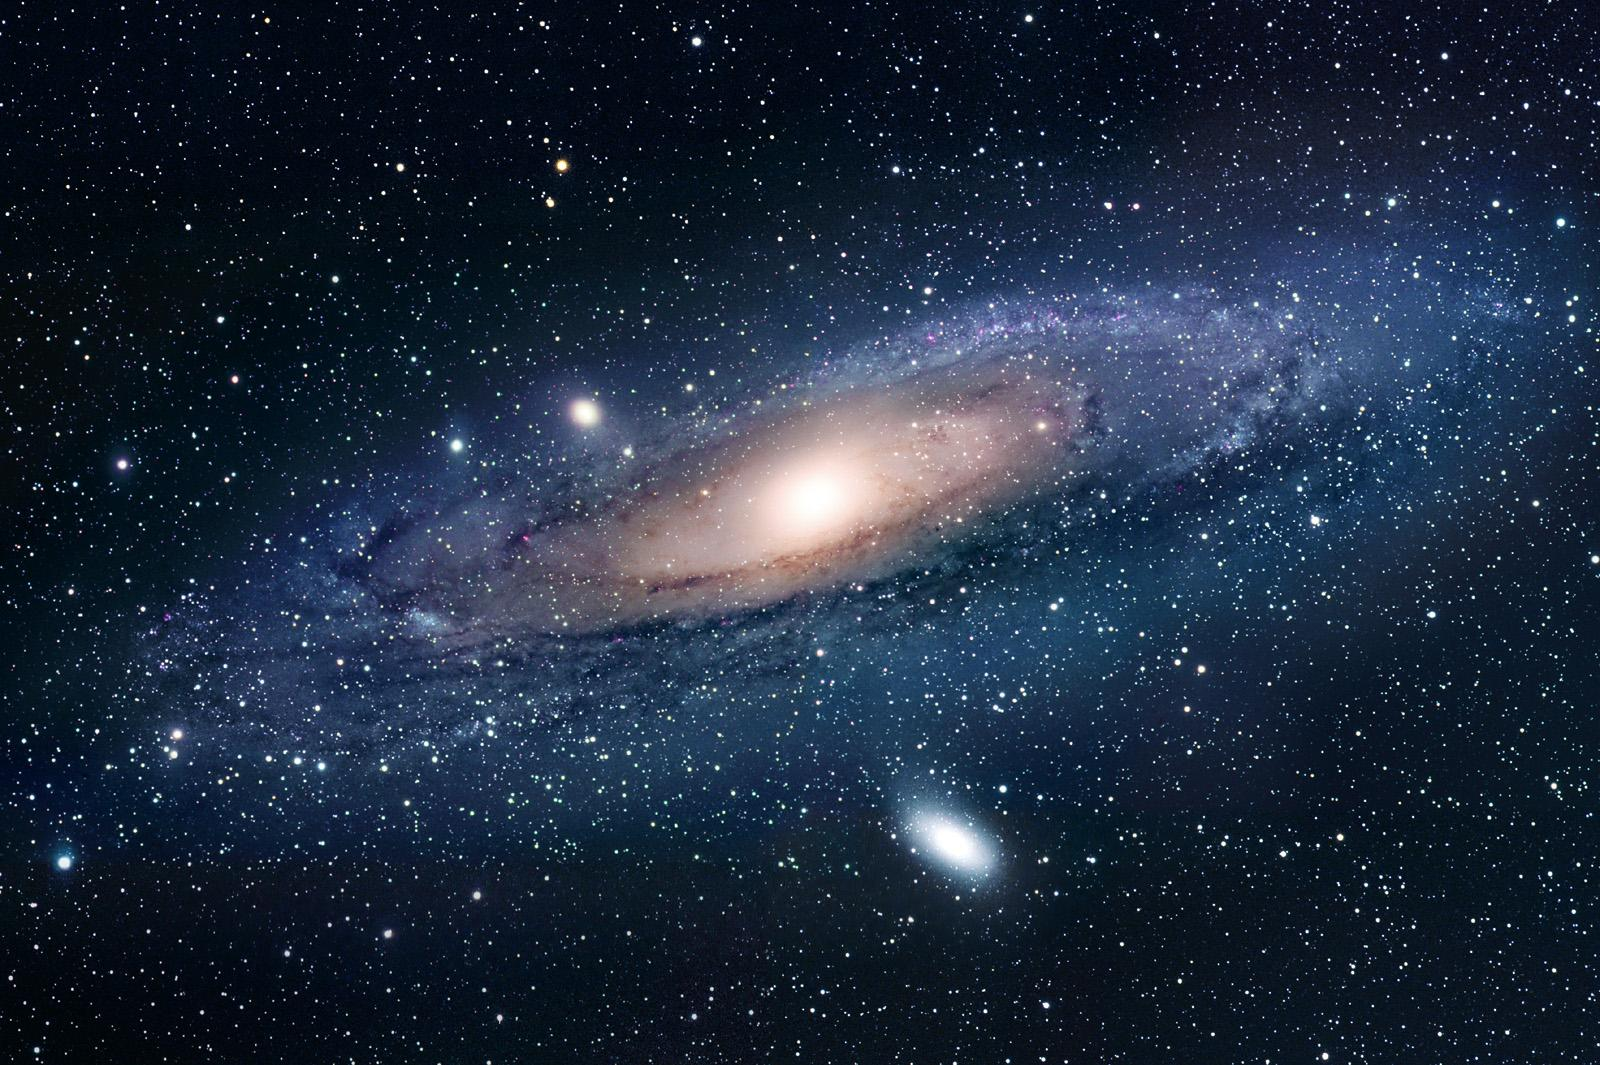
\includegraphics[width=0.75\textwidth]{res/sample-image.jpeg}
	\caption{A centered image}
	\label{fig::sample-label}
\end{figure}

\begin{figure}[h]
        % Rigth image
        \begin{subfigure}{0.45\textwidth}
        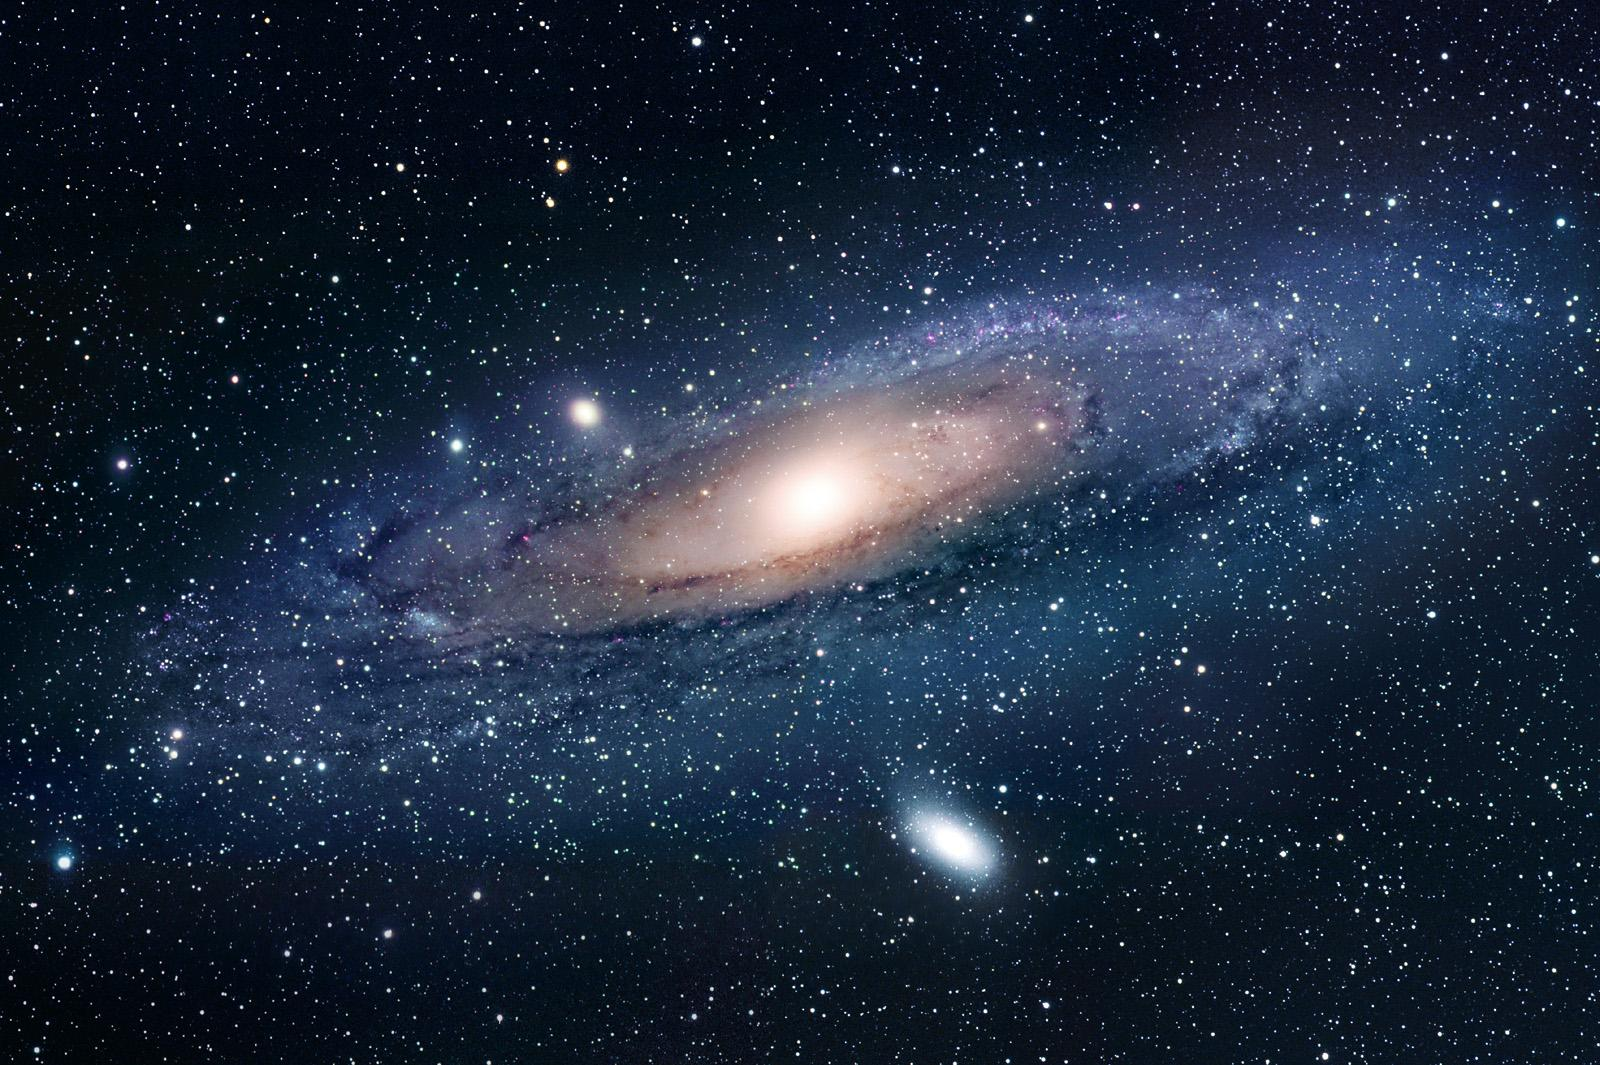
\includegraphics[width=1\linewidth]{res/sample-image.jpeg} 
        %\caption{Caption1}
        %\label{fig:serial-solution}
        
    \end{subfigure}
        % left image
        \begin{subfigure}{0.45\textwidth}
        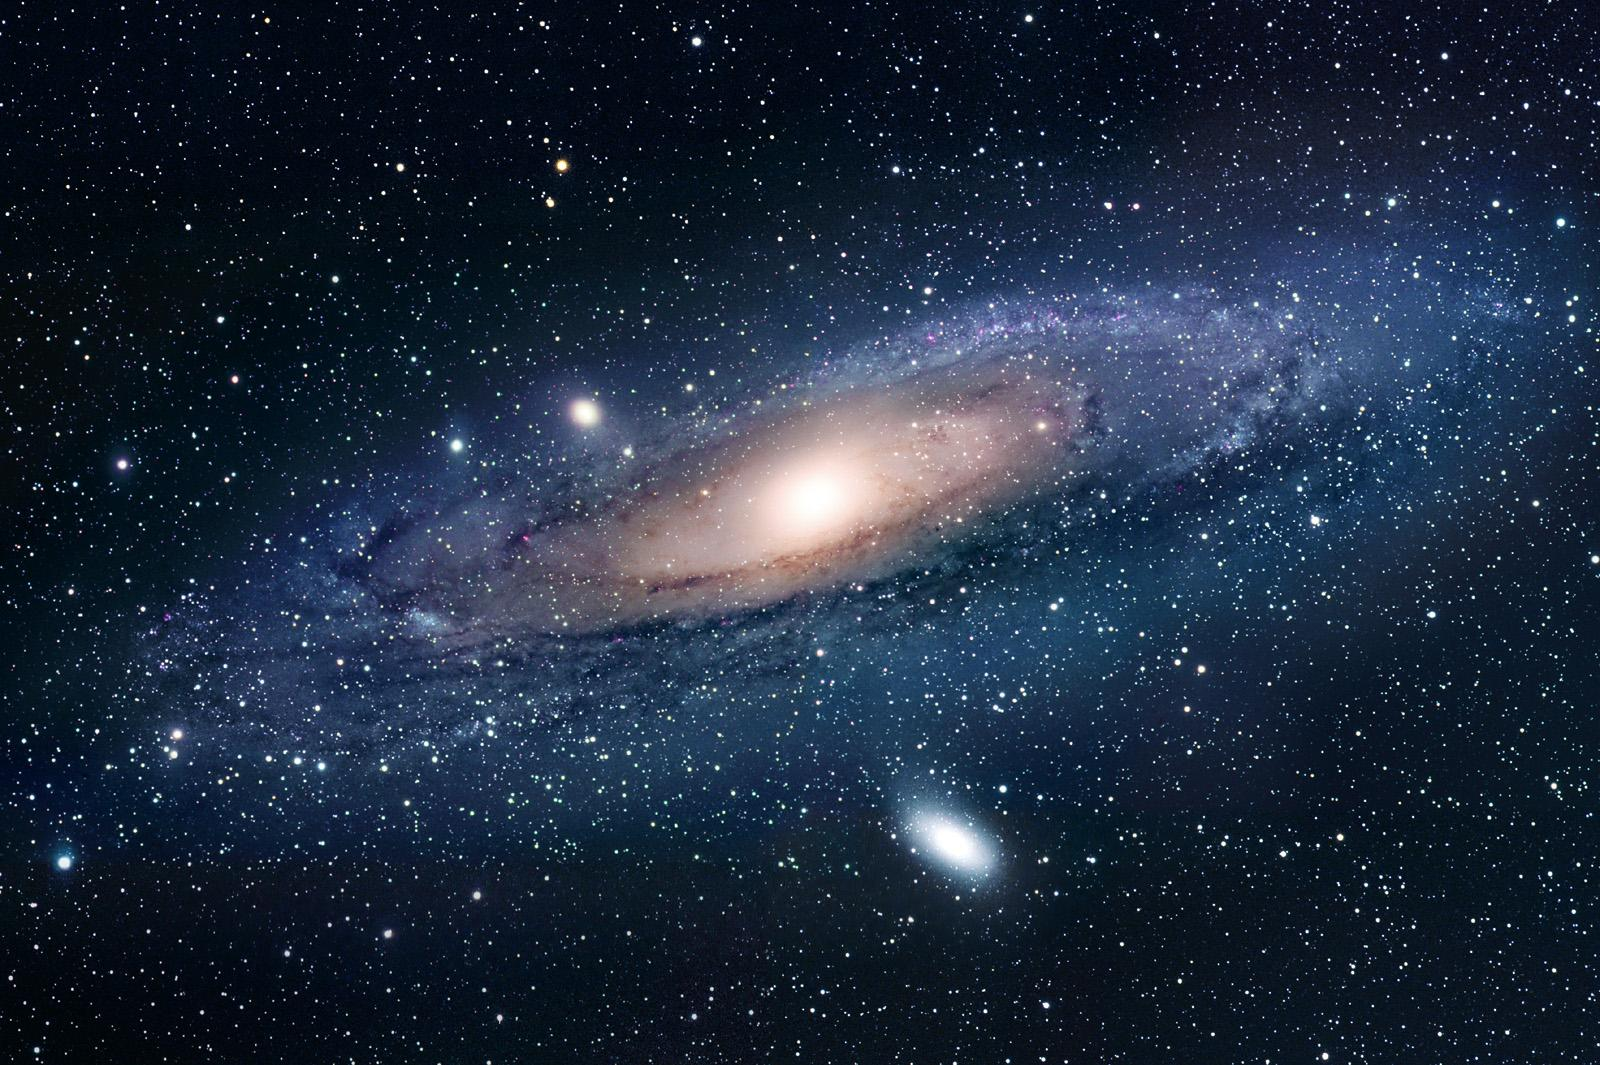
\includegraphics[width=1\linewidth]{res/sample-image.jpeg}
        %\caption{Caption 2}
        %\label{fig:parallel-solution}
    \end{subfigure}
    
    \caption{two images side-by-side}
    %\label{fig:serial-vs-parallel}
\end{figure}

\section{Is this just fantasy?}




%\begin{minipage}{\linewidth}
\begin{lstlisting}[caption={Sample Algorithm}]
int main()
{
    return 0;   // Comment
}
\end{lstlisting}
%\end{minipage}



\todo{remove sample chapter before release}


   
% \printbibliography
\end{document}